\documentclass[mathserif]{beamer}

\usetheme[secheader]{Madrid}
\setbeamercovered{transparent=50}

\usepackage{tikz}
\usetikzlibrary{trees}
\usepackage{url}

\usepackage{pygments}
\usepackage{graphicx}

\providecommand{\code}[1]{{\texttt{\scriptsize{#1}}}}
\providecommand{\inputcode}[1]{
  \begin{block}{}
    \scriptsize{\input{#1}}
  \end{block}
}

\title[Real World Moose]{Signatures, Moose, and MooseX::Declare\\For Real World Applications}
\author{Joel Berger}
\institute[UIC]{University of Illinois at Chicago}
\date{August 23, 2012}

\begin{document}

\begin{frame}
  \maketitle
\end{frame}

\begin{frame}{Outline}
  \tableofcontents
\end{frame}

\AtBeginSection{
  \begin{frame}{Outline}
    \tableofcontents[currentsection]
  \end{frame}
}

\section{Introduction}

\begin{frame}{Introduction}
  
\end{frame}

\section{\code{Method::Signatures}}

\begin{frame}{Introducing \texttt{Method::Signatures}}

A simple method \ldots

\vfill

\begin{columns}
  \begin{column}{0.49\linewidth}
    The old way:
    \inputcode{signatures/old}
  \end{column}
  \begin{column}{0.49\linewidth}
    The new way:
    \inputcode{signatures/new}
  \end{column}
\end{columns}
\end{frame}

\begin{frame}{More Fun}
  \inputcode{signatures/more}
\end{frame}

\section{\code{Moose}}

\begin{frame}{\texttt{Moose}}
  Like \code{Method::Signatures}, \code{Moose} makes object oriented code easier
  \inputcode{moose/person}
\end{frame}

\begin{frame}{Extending}
  \begin{itemize}
    \item Setup parent class using \code{extends}
    \item Modify attributes using \code{+} before name
    \item Modify methods using \code{before}, \code{after}, \code{override}, (\code{around}, \code{augment})
  \end{itemize}

  \inputcode{moose/soldier}
\end{frame}

\begin{frame}{Types}
  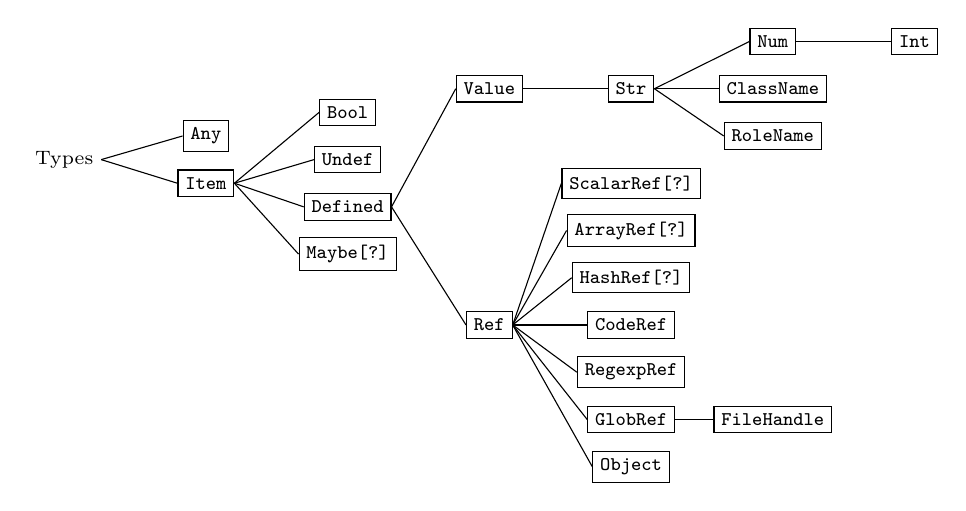
\begin{tikzpicture}
  \scriptsize
  \node {Types}[
      every node/.style={draw},
      grow via three points={
        one child at (1.8,0) and 
        two children at (1.8,0.3) and (1.8,-0.3)
      },
      edge from parent path={
        (\tikzparentnode.east) -- (\tikzchildnode.west)
      }
    ]
    child { node {\code{Any}}}
    child { node {\code{Item}}
      child { node {\code{Bool}}}
      child { node {\code{Undef}}}
      child { node {\code{Defined}}
        child { node {\code{Value}}
          child { node {\code{Str}}
            child { node {\code{Num}}
              child { node {\code{Int}}}
            }
            child { node {\code{ClassName}}}
            child { node {\code{RoleName}}}
          }
        }
        child[missing]{}
        child[missing]{}
        child[missing]{}
        child[missing]{}
        child { 
          node {\code{Ref}}
          child { node {\code{ScalarRef[?]}}}
          child { node {\code{ArrayRef[?]}}}
          child { node {\code{HashRef[?]}}}
          child { node {\code{CodeRef}}}
          child { node {\code{RegexpRef}}}
          child { node {\code{GlobRef}}
            child { node {\code{FileHandle}}}
          }
          child { node {\code{Object}}}
        }
      }
      child { node {\code{Maybe[?]}}}
    };
  \end{tikzpicture}
  \vfill
  Where \code{[?]} indicates an optional parameter, e.g. \code{ArrayRef[Int]}
\end{frame}

\section{\code{MooseX::Declare}}

\begin{frame}{\texttt{MooseX::Declare}}

\end{frame}

\section{My Research}

\begin{frame}{My Research}
  \begin{block}{}
    To be continued \ldots
  \end{block}
\end{frame}

\end{document}
